% 
% Lecture Template for ME3023 -  Measurements in Mechanical Systems - Tennessee Technological University
%
% Spring 2020 - Summer 2020
% Tristan Hill, May 07, 2020 - June 12, 2020 - July 08, 2020
% Module 6 - Steady State Circuits
% Topic 2 - Fundamental Laws
%

\documentclass{beamer}                         % for presentation (has nav buttons at bottom)
%\documentclass[handout]{beamer}  % for handout 
\usepackage{beamerthemesplit}
\usepackage{amsmath}
\usepackage{listings}
\usepackage{multicol}
\usepackage{framed}

\beamertemplateballitem

% custom colors
\definecolor{TTUpurple}{rgb}{0.3098, 0.1607, 0.5176} % TTU Purple (primary)
\definecolor{TTUgold}{rgb}{1.0000, 0.8666, 0.0000} % TTU Gold (primary) 
\definecolor{mygray}{rgb}{.6, .6, .6}
\definecolor{mypurple}{rgb}{0.6,0.1961,0.8}
\definecolor{mybrown}{rgb}{0.5451,0.2706,0.0745}
\definecolor{mygreen}{rgb}{0, .39, 0}
\definecolor{mypink}{rgb}{0.9960, 0, 0.9960}

% color commands
\newcommand{\R}{\color{red}}
\newcommand{\B}{\color{blue}}
\newcommand{\BR}{\color{mybrown}}
\newcommand{\K}{\color{black}}
\newcommand{\G}{\color{mygreen}}
\newcommand{\PR}{\color{mypurple}}
\newcommand{\PN}{\color{mypink}}
\newcommand{\OR}{\color{TTU}}
\newcommand{\GD}{\color{TTUgold}}


\setbeamercolor{palette primary}{bg=TTUpurple,fg=TTUgold}
\setbeamercolor{palette secondary}{bg=black,fg=TTUgold}
\setbeamercolor{palette tertiary}{bg=black,fg=TTUpurple}
\setbeamercolor{palette quaternary}{bg=TTUgold,fg=black}
\setbeamercolor{structure}{fg=TTUpurple} % itemize, enumerate, etc
\setbeamercolor{section in toc}{fg=TTUpurple} % TOC sections

%\usefonttheme{professionalfonts}

\newcommand{\Lagr}{\mathcal{L}} % lagrangian

\newcommand{\hspcu}{\underline{\hspace{20mm}}} % large horizontal space w underline
\newcommand{\vspccc}{\vspace{6mm}\\} % large vertical space
\newcommand{\vspcc}{\vspace{4mm}\\}   % medium vertical space
\newcommand{\vspc}{\vspace{2mm}\\}     % small vertical space

\newcommand{\hspcccc}{\hspace{10mm}} % large horizontal space
\newcommand{\hspccc}{\hspace{6mm}} % large horizontal space
\newcommand{\hspcc}{\hspace{4mm}}   % medium horizontal space
\newcommand{\hspc}{\hspace{2mm}}     % small horizontal space

\newcommand{\eqscl}{0.9}     % small horizontal space


\author{ME3023 - Measurements in Mechanical Systems} % original formatting from Mike Renfro, September 21, 2004

\newcommand{\MNUM}{6\hspace{2mm}} % Module number
\newcommand{\TNUM}{2\hspace{2mm}} % Topic number 
\newcommand{\moduletitle}{Steady State Circuits}
\newcommand{\topictitle}{Fundamental Laws} 

\newcommand{\sectiontitleI}{Ohm's Law}
\newcommand{\sectiontitleII}{Combining Resistance}
\newcommand{\sectiontitleIII}{Kirchhoff's Laws}
\newcommand{\sectiontitleIV}{Power Dissipation}

% custom box
\newsavebox{\mybox}

\title{Module \MNUM - \moduletitle}

\date{Mechanical Engineering\vspc Tennessee Technological University}

\begin{document}

\lstset{language=MATLAB,basicstyle=\ttfamily\small,showstringspaces=false}

\frame{\titlepage \center\begin{framed}\Large \textbf{Topic \TNUM - \topictitle}\end{framed} \vspace{5mm}}

% Section 0: Outline
\frame{

\large \textbf{Topic \TNUM - \topictitle} \vspace{3mm}\\


\begin{itemize}

	\item \sectiontitleI    \vspc % Section I
	\item \sectiontitleII 	\vspc % Section II
	\item \sectiontitleIII 	\vspc %Section III
	\item \sectiontitleIV 	\vspc %Section IV

\end{itemize}

}

% Section I:
\section{\sectiontitleI}

% Section I - Frame I:
\frame{ \small
\frametitle{\sectiontitleI}

\begin{multicols}{3}

{\bf James Maxwell}
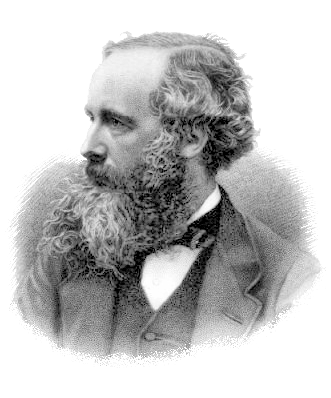
\includegraphics[scale=.30]{James_Clerk_Maxwell.png} \hspace{3mm}	

{\bf George Ohm} 
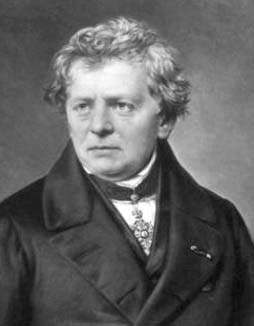
\includegraphics[scale=.30]{George_Ohm.png}	

{\bf Ohm's Notebook}
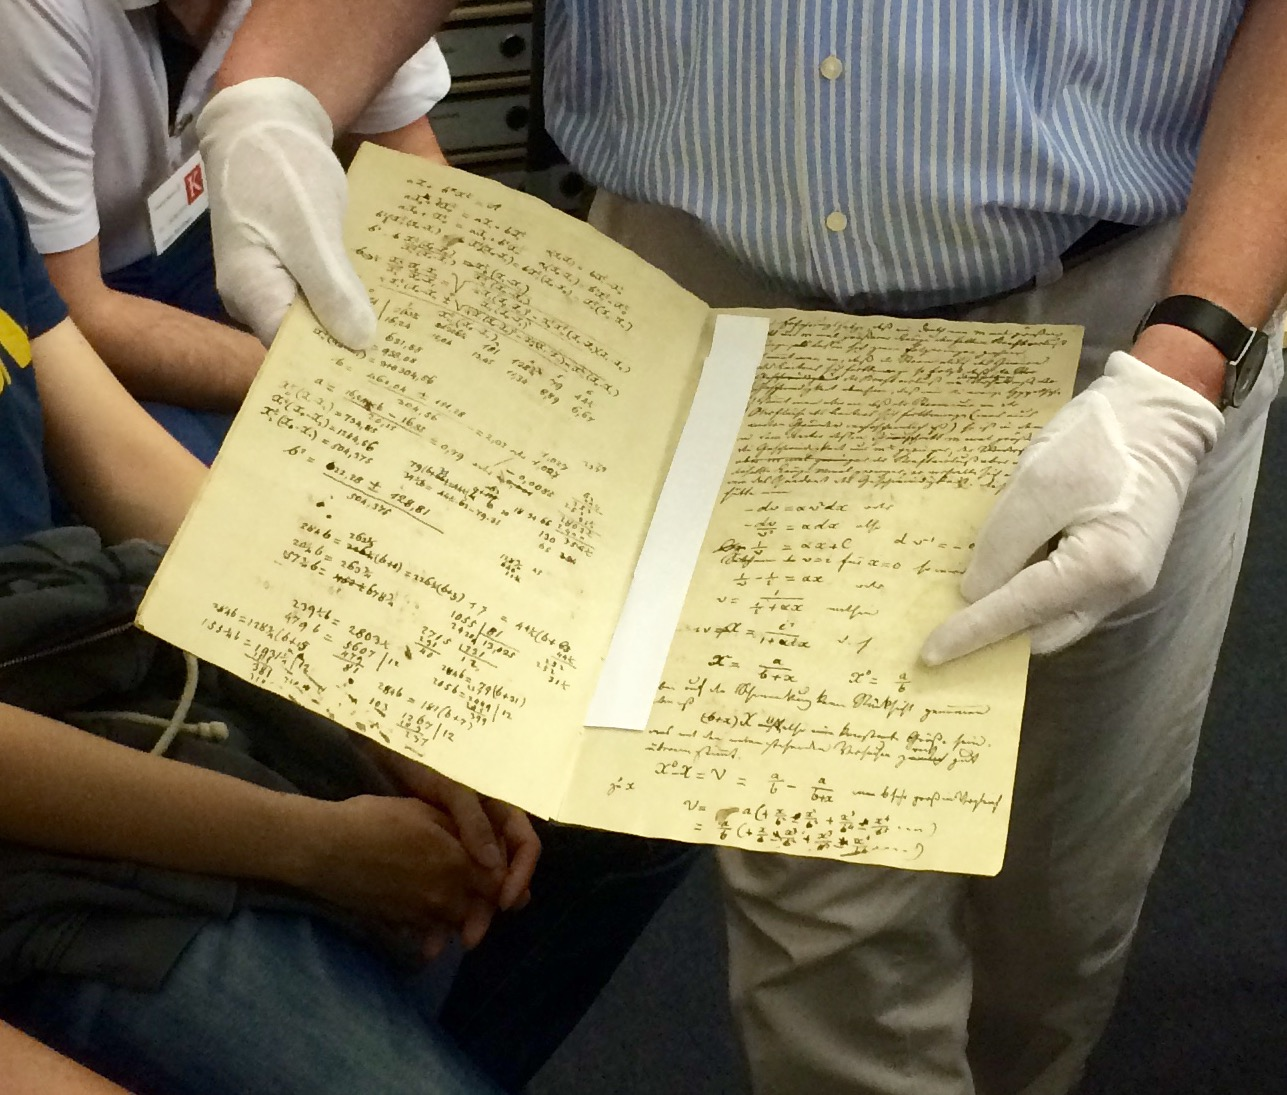
\includegraphics[scale=.07]{Ohms_Laborbuch.jpg}	

\end{multicols}
Ohm did his work on resistance in the years 1825 and 1826, and published his results in 1827 as the book Die galvanische Kette, mathematisch bearbeitet...
}

% Section I - Frame II:
\frame{ \small
\frametitle{\sectiontitleI}
Ohm's law states that the current through a conductor between two points is directly proportional to the voltage across the two points. 

\begin{multicols}{2}

\[ I=\frac{V}{R}  \] \vspace{1mm}\\
It is more commonly shown in the following form.
\[ V=IR \]

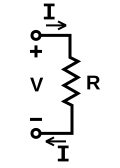
\includegraphics[scale=.8]{OhmsLaw.png}

\end{multicols}

}


% Section II:
\section{\sectiontitleII}

% Section II - Frame I:
\frame{
\frametitle{\sectiontitleII}
\begin{multicols}{2}

\begin{center}
Resistors in Series\vspcc
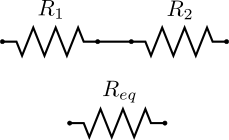
\includegraphics[scale=.2]{series_resistors.png} 
\end{center}
\[R_{eq}=R_1+R_2 \]
\vspace{15mm}\\

\begin{center}
Resistors in Parallel \vspcc
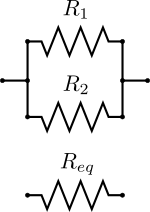
\includegraphics[scale=.2]{parallel_resistors.png}
\end{center}
\[R_{eq}=\frac{1}{\frac{1}{R_1}+\frac{1}{R_2}} \]
\vspace{10mm}\\

\end{multicols}

}


% Section III:
\section{\sectiontitleIII}

% Section III - Frame I:
\frame{ \small
\frametitle{\sectiontitleIII}

Both of Kirchhoff's laws can be understood as corollaries of Maxwell's equations in the low-frequency limit. They are accurate for DC circuits, and for AC circuits at frequencies where the wavelengths of electromagnetic radiation are very large compared to the circuits. \vspc 

\begin{enumerate}
\item Kichhoff's Voltage Law (KVL)
\item Kichhoff's Current  Law (KCL)
\end{enumerate}

}

% Section III - Frame II:
\frame{ \small
\frametitle{\sectiontitleIII}

\begin{multicols}{2}
{\bf Kichhoff's Voltage Law (KVL)} - The sum of the voltages around a loop (aka mesh) equals zero.\\ $ \sum\limits_{k=1}^{n} v_k = 0 $ \\
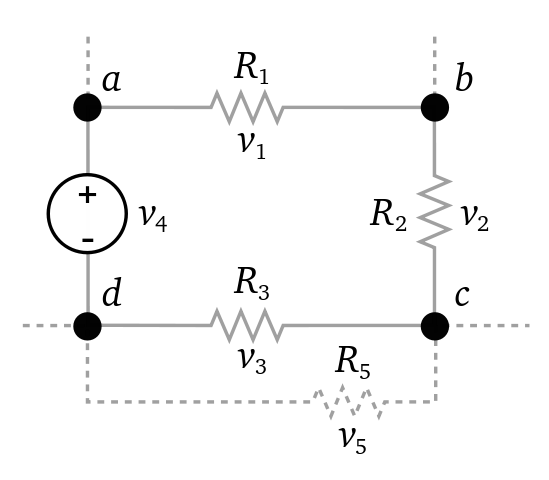
\includegraphics[scale=.20]{Kirchhoffs_voltage_law.png} 

{\bf Kichhoff's Current  Law (KCL)} - The sum of the current flowing in and out of  node (aka junction) equals zero. \\ $ \sum\limits_{k=1}^{n} i_k = 0 $ \vspace{2mm}\\
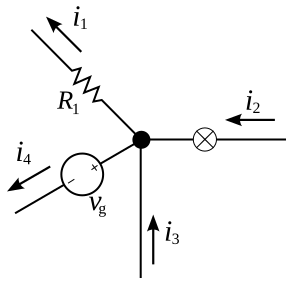
\includegraphics[scale=.4]{Kirchhoffs_current_law.png} 
\end{multicols}

}

%% Section IV:
\section{\sectiontitleIV}

% Section IV - Frame I:
\frame{ \small
\frametitle{\sectiontitleIV}
	Energy is transformed in to heat in passive circuit components. For a resistor the power dissipation can be found with following relations. \vspace{5mm}
	
	$P=IV$ \hspace{20mm} $V=IR$
}
	
% Section IV - Frame II:
\frame{ \small
\frametitle{\sectiontitleIV}

	Power is the rate of energy dissipated, aka the amount of energy lost per unit of time. How do we compute total energy for the power? 
	
	\[E=\int\limits_{t1}^{t2}Pdt \]  
}


\end{document}





